%-*- coding: utf-8 -*-
\textcolor[RGB]{46, 116, 181}{\chapter{Élaboration}}
\section{Planification des activités}
Nous fixons la date de livraison à 2 semaines avant la présentation. La présentation du projet étant prévue pour le 14/09/2017; notre date de livraison est donc le \textbf{31/08/2017}. Entre le 4 mars et le 31 août, il y a 181 jours moins 7 jours fériés, nous disposons donc de \textbf{174 jours}.

Nous avons identifié huit étapes de développement:
\begin{itemize}
	\item Analyse des exigences
	\item Cas d'utilisation
	\item Modèle de domaine.
	\item Séquences système
	\item Classes participantes.
	\item Diagramme d'interactions.
	\item Classes de conception.
	\item Code.
\end{itemize}
Pour évaluer la part de chaque étapes de développement, nous nous basons sur l'affirmation suivante \enquote{Aujourd'hui, un projet c'est 80\% de réflexion et 20\% de développement} (voir \url{http://www.logadap.fr/methodologie-creation-logiciel/}). Ainsi, le code va occuper 20\% de notre temps, soit 35 jours; reste 139 jours à répartir entre les 7 étapes précédentes, soit 20 jours chacunes.
Le diagramme de GANTT est donc le suivant:
\begin{figure}[H]
\label{Gantt}
  \centering
      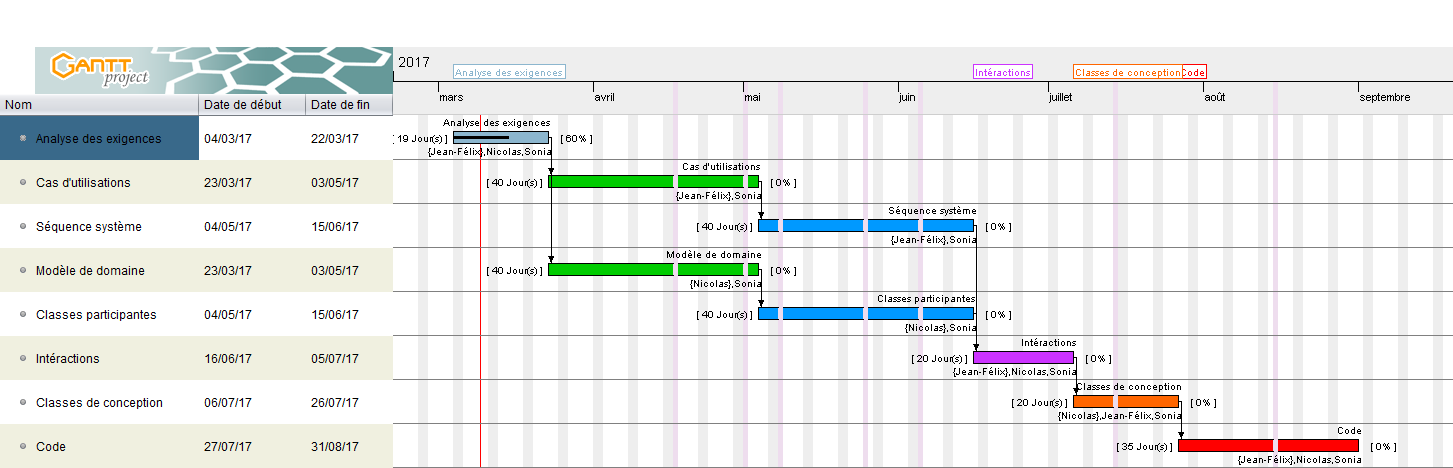
\includegraphics[width=1.0\textwidth]{Vitameal_gantt} %
\caption{Gantt}
\end{figure}

Le diagramme de PERT donne une autre vues de la répartition et de l'enchaînement des taches:
\begin{figure}[H]
\textbf{P}rogram \textbf{E}valuation and \textbf{R}eview \textbf{T}echnique
\label{PERT}
  \centering
      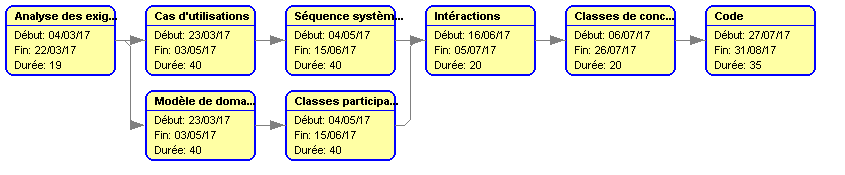
\includegraphics[width=1.0\textwidth]{Vitameal_pert} %
\caption{PERT}
\end{figure}

\section{Affectation des ressources}
Les ressources sont affectées comme suit:

\begin{tabular}{|l|l|}
\hiderowcolors
  \hline
  Tâches & Ressources \\ \hline
  Analyse des exigences & Nicolas, Sonia, Jean-Félix \\
  Cas d'utilisation & Jean-Félix 67\%, Sonia 33\% \\
  Modèle de domaine & Nicolas 67\%, Sonia 33\% \\
  Séquences système & Jean-Félix 67\%, Sonia 33\% \\
  Classes participantes & Nicolas 67\%, Sonia 33\% \\
  Diagramme d'interactions & Nicolas, Sonia, Jean-Félix \\
  Classes de conception & Nicolas, Sonia, Jean-Félix \\
  Code & Nicolas, Sonia, Jean-Félix \\ \hline
\end{tabular}

\begin{figure}[H]
\label{Ressources}
  \centering
      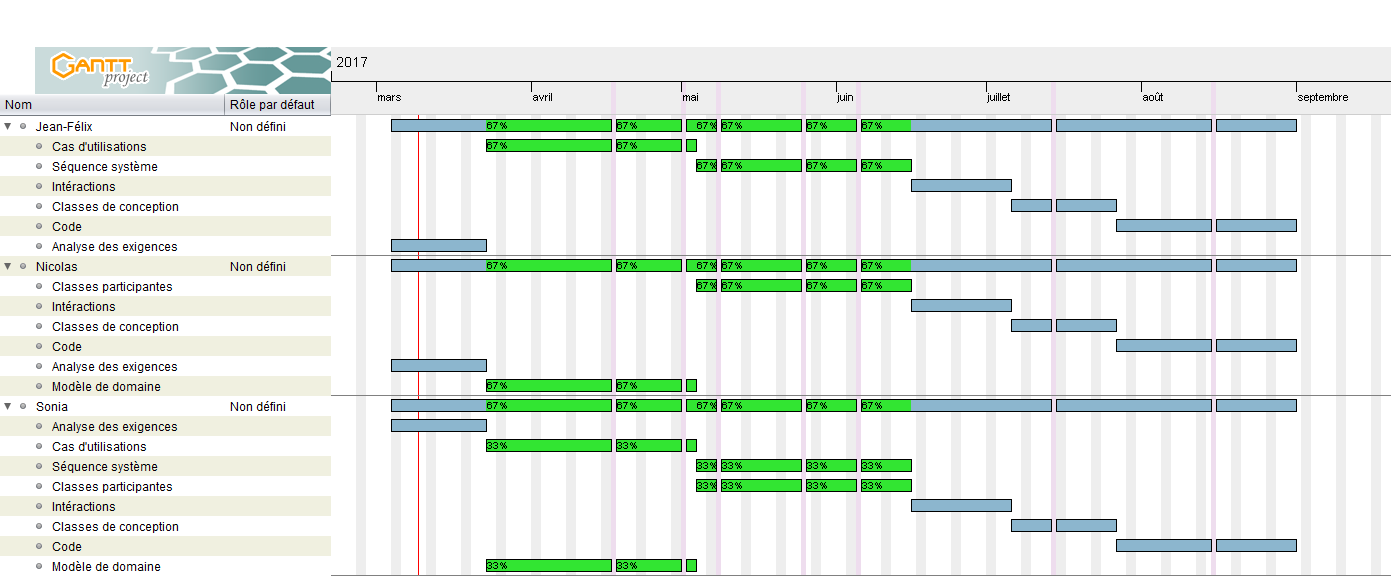
\includegraphics[width=1.0\textwidth]{Vitameal_ressources} %
\caption{Ressources}
\end{figure}

\section{Description de l'usine logicielle}

L'usine logicielle de Vitameal répond aux exigences suivantes :

\begin{itemize}
	\item respecter les règles de qualités ;
	\item avoir une documentation claire et intégrée au projet ;
	\item gérer les erreurs et assurer leurs suivies ;
	\item versionnionner le code source et la documentation ;
	\item avoir un espace commun accessible à distance ;
	\item gérer un espace de livraison générant des indicateurs de santé sur le projet ;
	\item avoir un outil de conception UML couvrant la methode minimal UML ;
	\item gérer la planification du projet.
\end{itemize}

\subsection{Outils utilisés}

Les outils utilisés par l'usine logicielle de Vitameal se sépare en deux catégories :

\begin{itemize}
	\item Le côté poste de développement qui correspond aux outils installés par chaque développeur sur sa machine ;
	\item Le côté espace d'intégration continue et de gestion de projet qui correspond aux outils composant l'espace communs de collaborations.
\end{itemize}

La documentation du projet est assurée par l'utilisation de la syntaxe \emph{markdown} intégrée à l'outil \emph{GitHub} et le langage de génération des livrables est \emph{LaTex}.

Le langage cible de cette usine est Java, mais elle peut facilement être adaptée à d'autre langage.

\subsubsection{Côté poste de développement}

\begin{itemize}
	\item \textbf{Eclipse} comme IDE pour écrire/éditer le code de l'application ;
	\item \textbf{Maven} comme constructeur du projet (gestion des dépendances, automatisation de la construction ;
	\item \textbf{JUnit} pour écrire les tests unitaires de l'application et \textbf{Codertura} pour analyser la couverture du projet par ces tests ;
	\item \textbf{Git} pour versionner les sources du projet ;
	\item \textbf{Papyrus} pour modéliser selon le standard UML le projet ;
	\item \textbf{GanttProject} pour planifier le projet avec un diagramme de Gantt ;
	\item \textbf{TEXMaker} pour éditer les fichiers\texttt{.tex} avec un comportement proche des \emph{WYSIWYG} (optionnel).
\end{itemize}

\subsubsection{Côté espace d'intégration continue et gestion de projet}

\begin{itemize}
	\item \textbf{GitHub} comme gestionnaire à distance du repositorie Git principal, comme tracker de bug et comme affichage visuel des taches à faire ;
	\item \textbf{Redmine} pour organiser le projet et rendre visible l'avancement du projet;
	\item \textbf{Jenkins} comme serveur d'intégration continue ;
	\item \textbf{SonarQube} comme analyseur de qualité du code.
\end{itemize}

\subsection{Schema de fonctionnement}

\begin{figure}[H]
	\label{Usine logicielle de Vitameal}
	\centering
	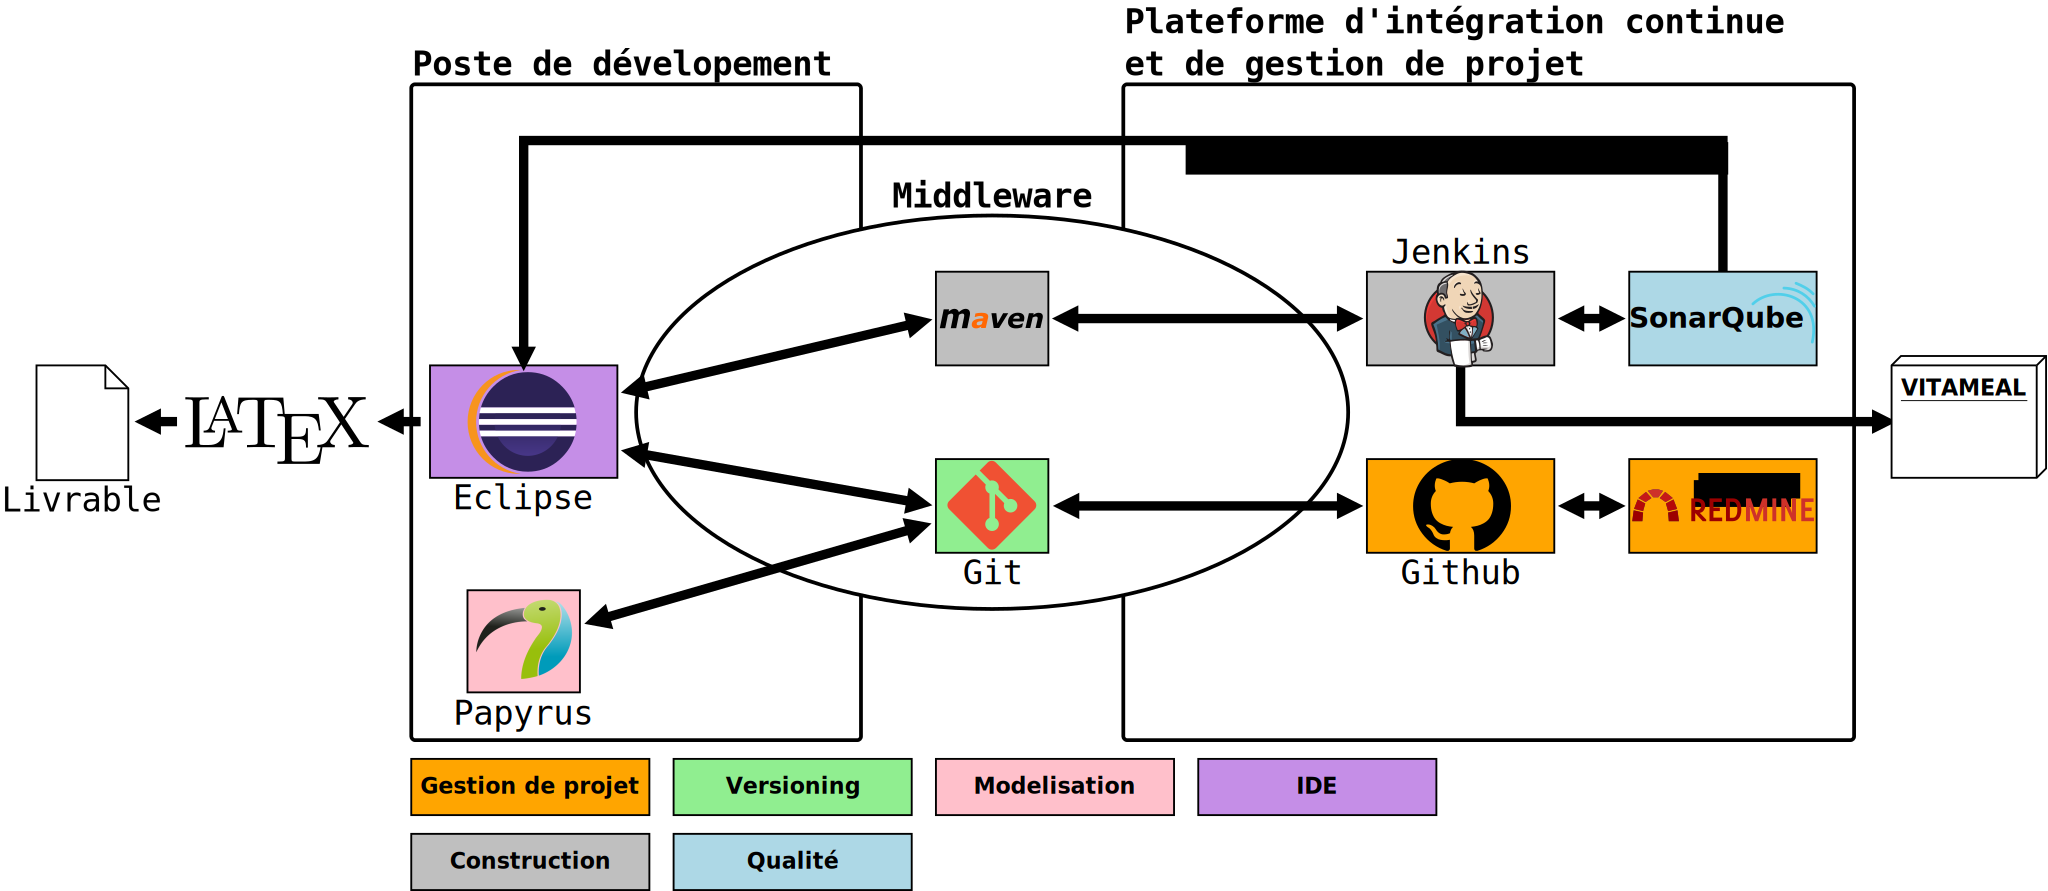
\includegraphics[width=0.8\textwidth]{usine_vitameal} %
	\caption{Usine logicielle de Vitameal}
\end{figure}


L'usine logicielle du projet Vitameal à pour porte d'entrée principale L'IDE  \textbf{Eclipse}, qui munis de plugins adéquat permet d'éditer la plupart des fichiers composants le projet.  
La collaboration sur le projet est assurée par le gestionnaire de version  \textbf{Git}, avec un repositorie central hébergé par \textbf{GitHub}.

Le  \textit{feedback} sur la santé du projet (qualité, couverture par les tests, build réussi, ...) est géré par le serveur d'intégration continue  \textbf{Jenkins}, utilisant \textbf{Maven} comme outils de configurations du projet et se branchant sur \textbf{SonarQube} pour obtenir les métriques.

L' outil  \textbf{Papyrus} est dédié à la conception UML de l'application, et l'outil  \textbf{Redmine} à la gestion de l'avancement du projet.

\section{\colorbox{yellow}{TODO} Analyse}

\section{\colorbox{yellow}{TODO} Vision détaillée}

\section{\colorbox{yellow}{TODO} Cible}

\section{\colorbox{yellow}{TODO} Risques}

\section{\colorbox{yellow}{TODO} Besoins précis}

\section{\colorbox{yellow}{TODO} Définition itérative de l'architecture}

\section{\colorbox{yellow}{TODO} Estimation fine}
